\documentclass[14pt,a4paper]{scrartcl}
\usepackage{cmap}
\usepackage[utf8]{inputenc}
\usepackage[T1,T2A]{fontenc}
\usepackage[english,russian]{babel}
\usepackage{relsize}
\usepackage{graphicx}
\usepackage{subfigure}
\usepackage{mathtools}
\usepackage{amssymb}
\usepackage{float}
\usepackage{sidecap}
\usepackage{wrapfig}
\usepackage{caption}
\usepackage[table,xcdraw]{xcolor}
\usepackage{minted}
\begin{document}
	\begin{titlepage}
	\begin{center}
		\large
		МИНИСТЕРСТВО ОБРАЗОВАНИЯ И НАУКИ\\ РОССИЙСКОЙ ФЕДЕРАЦИИ
		
		\vspace{0.5cm}
		
		МГТУ им Н.Э.Баумана
		\vspace{0.25cm}
		
		Факультет ФН
		
		Кафедра вычислительной математики и математической физики
		\vfill
		
		
		Соколов Арсений Андреевич\\
		\vfill
		
		
		{\LARGE Домашнее задание №1 по теории случайных процессов\\[2mm]
		}
		\bigskip
		
		3 курс, группа ФН11-63Б\\
		Вариант 19
	\end{center}
	\vfill
	
	\newlength{\ML}
	\settowidth{\ML}{«\underline{\hspace{0.7cm}}» \underline{\hspace{2cm}}}
	\hfill\begin{minipage}{0.4\textwidth}
		Преподаватель\\
		\underline{\hspace{3cm}} Т.\,В.~Облакова\\
		«\underline{\hspace{0.7cm}}» \underline{\hspace{1.71cm}} 2019 г.
	\end{minipage}%
	\bigskip
	
	
	\vfill
	
	\begin{center}
		Москва, 2019 г.
	\end{center}
\end{titlepage}

\section*{Начальные данные}

\begin{minted}{R}
> ### Начальные данные:
> m <- 6 # Число состояний марковской цепи
> k <- 5 # время (шаги)
> n <- 180 # траектории
\end{minted}

\section*{Задание 1}

Смоделировать вектор начальных вероятностей $(p(0)) = \vec{p}(0)$ и матрицу переходных вероятностей $P$ для однородной цепи Маркова с данным числом состояний ${s_1,s_2,…,s_m}$.\\
\textbf{Решение.}\\
1. Генерируем $(m+1)$ раз вектор $\vec{r}=(r_1,r_2,…,r_{m-1})$ из независимых и равномерно распределенных на отрезке $[0,1]$ случайных величин.
\begin{minted}{R}
> r_tmp <- replicate((m+1), runif((m-1), min = 0, max = 1), simplify = F)
> r_tmp
[[1]]
[1] 0.6851245 0.1042469 0.8278534 0.6700496 0.8882372

[[2]]
[1] 0.5553275 0.2135837 0.4276684 0.4595399 0.6044195

[[3]]
[1] 0.8445415 0.6948895 0.7662574 0.5193746 0.7318254

[[4]]
[1] 0.63079243 0.30112912 0.02484105 0.23813089 0.02754031

[[5]]
[1] 0.3608469 0.1258250 0.6258345 0.7741952 0.4322131

[[6]]
[1] 0.84741511 0.07761379 0.81335679 0.47664151 0.57196036

[[7]]
[1] 0.1927269 0.7714035 0.8828472 0.8983539 0.7973951
\end{minted}


2. Для каждого из полученный векторов строим вариационный ряд, то есть упорядочиваем по возрастанию.

\begin{minted}{R}
> r <- lapply(r_tmp, sort)
> r
[[1]]
[1] 0.1042469 0.6700496 0.6851245 0.8278534 0.8882372

[[2]]
[1] 0.2135837 0.4276684 0.4595399 0.5553275 0.6044195

[[3]]
[1] 0.5193746 0.6948895 0.7318254 0.7662574 0.8445415

[[4]]
[1] 0.02484105 0.02754031 0.23813089 0.30112912 0.63079243

[[5]]
[1] 0.1258250 0.3608469 0.4322131 0.6258345 0.7741952

[[6]]
[1] 0.07761379 0.47664151 0.57196036 0.81335679 0.84741511

[[7]]
[1] 0.1927269 0.7714035 0.7973951 0.8828472 0.8983539
\end{minted}

3. Находим длины отрезков, на которые вектор $\vec{r}$ разбивает отрезок $[0;1]$ -- получаем вектор вероятностей $\vec{p}$.

\begin{minted}{R}
> p_tmp <- lapply(r, diff)
> 
> heads <- lapply(r, head, 1)
> tails <- lapply(r, function(x) (1-tail(x,1)))
> 
> p <- mapply(append, mapply(append, heads,p_tmp,SIMPLIFY = F),
+             tails, SIMPLIFY = F)
> p
[[1]]
[1] 0.10424689 0.56580266 0.01507492 0.14272891 0.06038386 0.11176275

[[2]]
[1] 0.21358371 0.21408467 0.03187156 0.09578759 0.04909199 0.39558049

[[3]]
[1] 0.51937464 0.17551486 0.03693588 0.03443202 0.07828406 0.15545854

[[4]]
[1] 0.024841045 0.002699268 0.210590575 0.062998231 0.329663308 0.369207573

[[5]]
[1] 0.12582500 0.23502193 0.07136614 0.19362140 0.14836075 0.22580478

[[6]]
[1] 0.07761379 0.39902772 0.09531885 0.24139643 0.03405832 0.15258489

[[7]]
[1] 0.19272691 0.57867661 0.02599155 0.08545218 0.01550662 0.10164613
\end{minted}

Проверим, что полученный вектора обладают свойством стохастичности:

\begin{minted}{R}
> sapply(sum, p)
[1] 1 1 1 1 1
\end{minted}

Получили, что сумма элементов каждого вектора $\vec{p}$ равна единице.

4. Первый из полученных векторов $\vec{p}$ считаем вектором начальных вероятностей, из остальных составляем матрицу переходов $P$, записывая их по строкам.

\begin{minted}{R}
> p0 <- p[[1]] # вектор начальных условий
> p0
[1] 0.10424689 0.56580266 0.01507492 0.14272891 0.06038386 0.11176275
> P <- t(simplify2array(p))[-1,] # матрица переходов
> P
	[,1]        [,2]       [,3]       [,4]       [,5]      [,6]
[1,] 0.21358371 0.214084670 0.03187156 0.09578759 0.04909199 0.3955805
[2,] 0.51937464 0.175514856 0.03693588 0.03443202 0.07828406 0.1554585
[3,] 0.02484105 0.002699268 0.21059057 0.06299823 0.32966331 0.3692076
[4,] 0.12582500 0.235021926 0.07136614 0.19362140 0.14836075 0.2258048
[5,] 0.07761379 0.399027718 0.09531885 0.24139643 0.03405832 0.1525849
[6,] 0.19272691 0.578676610 0.02599155 0.08545218 0.01550662 0.1016461
\end{minted}

\pagebreak
\section*{Задание 2}
Построить размеченный граф состояний цепи.\\
\textbf{Решение.}\\

\begin{minted}{R}
> library(markovchain)
> library(diagram)
> 
> png(filename = "../img/1.png",
+     width = 1920, height = 1080,
+     res = 96 * 1.25)
> plotmat(signif(P,3), 
+         lwd = 1, box.lwd = 2, 
+         cex.txt = 0.8, 
+         box.size = 0.04, 
+         box.type = "circle", 
+         box.prop = 0.5,
+         box.col = "light blue",
+         arr.length=.25,
+         arr.width=.1,
+         self.cex = .7,
+         self.shifty = -.01,
+         self.shiftx = .07,
+         main = "Markov Chain")
> dev.off()
\end{minted}

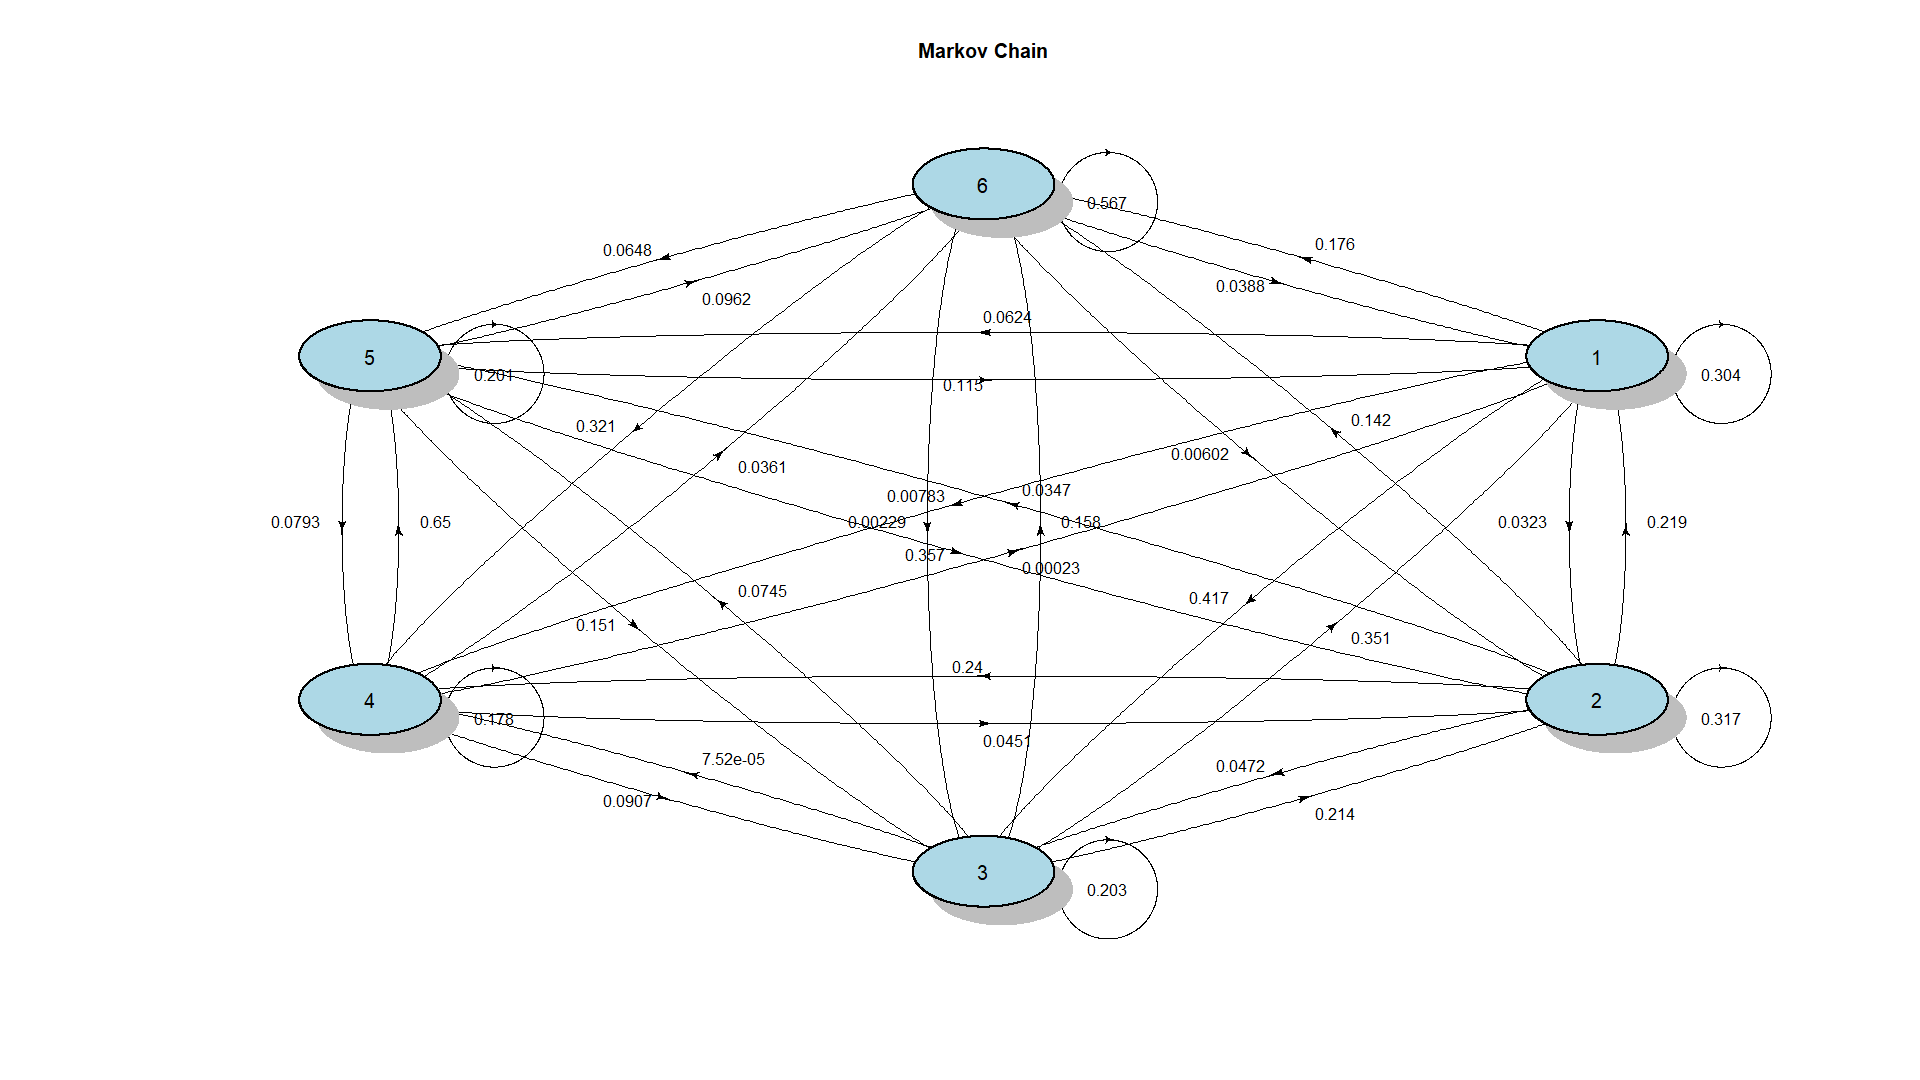
\includegraphics[angle=90,origin=t, scale=0.75]{../img/1.png}

\pagebreak

\section*{Задание 3.}
Вычислить безусловные вероятности состояний смоделированной цепи на k шаге.\\
\textbf{Решение.}\\

\begin{minted}{R}
> library(matrixcalc)
> p_k <- p0 %*% matrix.power(P,k)
> p_k
	[,1]      [,2]      [,3]       [,4]       [,5]     [,6]
[1,] 0.2696947 0.2897812 0.0490421 0.09383964 0.07187831 0.225764
\end{minted}


\section*{Задание 4}
Смоделировать $n$ траекторий полученной цепи за $k$ шагов и найти вектор относительных частот ее состояний на $k$ шаге.\\
\textbf{Решение.}\\

1. Генерируем равномерно распределенную на $[0;1]$ случайную величину $r_0$ и по вектору $r_1$ разыгрываем начальное состояние следующим образом: если $r_0 < r_{1_1}$, то полагаем, что $\xi_0 = s_1 = 1$, если $r_0 < r_{1_2}$, то полагаем, что $\xi_0 = s_2 = 2$, \ldots, если $r_0 < r_{1_{m-1}}$, то полагаем, что $\xi_0 = s_{m-1} = m-1$, иначе если $r_0 > r_{1_{m-1}}$, то полагаем, что $\xi_0 = s_{m} = m = j_0$.


\begin{minted}{R}
> r0 <- runif(1, min = 0, max = 1)
> r0
[1] 0.496682
> foo <- function(r0_loc,j)
+   {
+     ifelse(r0_loc < r[[j+1]][1],1,
+     ifelse(r0_loc < r[[j+1]][2],2,
+     ifelse(r0_loc < r[[j+1]][3],3,
+     ifelse(r0_loc < r[[j+1]][4],4,
+     ifelse(r0_loc < r[[j+1]][5],5,6)))))
+   }
>   
>   step_1 <- foo(r0,1)
> step_1
[1] 5
###
> r[[1]]
[1] 0.05178461 0.13461717 0.35892529 0.46682475 0.54672747
\end{minted}

Разыгранное число $r_0 = 0.496682$, что меньше, чем 5-эй элемент $r_1$, но больше, чем 4-эй, то есть $(0.46682475 = r_{1_4})< 0.496682 < (0.54672747 = r_{1_5})  \Rightarrow \xi_0 = 5$. \\

2. Генерируем ещё одно значение $r_1$ и по строке с номером $j_0 = 5$ аналогично предыдущему пункту разыгрываем значение $\xi_1:$

\begin{minted}{R}
> r_1 <- runif(1, min = 0, max = 1)
> r_1
[1] 0.8652293
> step_2 <- foo(r_1,step_1)
> step_2
[1] 5
\end{minted}

3. Повторяем алгоритм  заданное число раз $k$.

\begin{minted}{R}
> r_2 <- runif(1, min = 0, max = 1)
> r_2
[1] 0.2317151
> step_3 <- foo(r_2,step_2)
> step_3
[1] 2

> r_3 <- runif(1, min = 0, max = 1)
> r_3
[1] 0.05540007
> step_4 <- foo(r_3,step_3)
> step_4
[1] 1

> r_4 <- runif(1, min = 0, max = 1)
> r_4
[1] 0.08274597
> step_5 <- foo(r_4,step_4)
> step_5
[1] 1
\end{minted}

Получаем выборочную траекторию цепи:

\begin{minted}{R}
> c(step_1,step_2,step_3,step_4,step_5)
[1] 5 5 2 1 1
\end{minted}
	
4. Повторяем процедуру 1-3 $n$ число раз.

В общем виде алгоритм выглядит следующим образом:
\begin{minted}{R}
tracs <- list()

for (k in 1:n)
{
	r0 <- runif(1, min = 0, max = 1)
	foo <- function(r0_loc,j)
	{
		ifelse(r0_loc < r[[j+1]][1],1,
		ifelse(r0_loc < r[[j+1]][2],2,
		ifelse(r0_loc < r[[j+1]][3],3,
		ifelse(r0_loc < r[[j+1]][4],4,
		ifelse(r0_loc < r[[j+1]][5],5,6)))))
	}
	
	step_1 <- foo(r0,0)
	step_2 <- foo(runif(1, min = 0, max = 1),step_1)
	step_3 <- foo(runif(1, min = 0, max = 1),step_2)
	step_4 <- foo(runif(1, min = 0, max = 1),step_3)
	step_5 <- foo(runif(1, min = 0, max = 1),step_4)
	
	trac <- list(c(step_1,step_2,step_3,step_4,step_5))
	tracs[k] <- trac
}

tracs_array <- t(simplify2array(tracs,higher = F))
colnames(tracs_array) <- c("Шаг 1","Шаг 2","Шаг 3","Шаг 4","Шаг 5")
rownames(tracs_array) <- paste("Тр.",as.character(1:n))
\end{minted}

В итоге получаем $n=180$ штук траекторий длины $k=5$.

Посмотрим на первые и последние 10 траекторий:

\begin{minted}{R}
> head(tracs_array,10)
Шаг 1 Шаг 2 Шаг 3 Шаг 4 Шаг 5
Тр. 1      3     2     1     1     1
Тр. 2      2     3     6     2     1
Тр. 3      3     3     3     5     2
Тр. 4      1     1     1     3     6
Тр. 5      3     2     3     2     5
Тр. 6      3     3     6     2     1
Тр. 7      1     1     4     4     4
Тр. 8      3     5     2     6     1
Тр. 9      3     2     3     2     4
Тр. 10     1     3     2     1     3
> tail(tracs_array,10)
Шаг 1 Шаг 2 Шаг 3 Шаг 4 Шаг 5
Тр. 171     1     1     3     6     1
Тр. 172     1     1     3     2     4
Тр. 173     2     4     1     1     3
Тр. 174     3     6     6     6     2
Тр. 175     3     5     3     6     2
Тр. 176     5     5     5     3     2
Тр. 177     2     5     4     4     1
Тр. 178     1     1     1     3     3
Тр. 179     3     5     3     2     2
Тр. 180     3     3     4     4     1
\end{minted}

















\end{document}